%!TEX encoding = IsoLatin

%% Document is article 
\documentclass[a4paper]{article}

%% ----------------------------------------------------- PACKAGES ----------------------------------------------------- %%
\usepackage{coolArticle}

%% ---------------------------------------------------- DOCUMENT ---------------------------------------------------- %%
\begin{document}

\noindent \textsc{Gallos-Montbrun} Gr�goire\\
\textsc{Faury} Louis 
\vspace{15pt}

	\titlebox{0.6}{\Large Model Predictive Control}{\Large \textbf{\textcolor{blue}{Building Temperature Regulation}}}
	
	\section{Introduction}
	{
		\paragraph{} This project aims at controlling the temperature inside a 3 room building. The full state and output dynamics are given by : 
		\begin{equation}
			\begin{aligned}
				x^+ &= Ax + B_uu + B_dd\\
				y &= Cx
			\end{aligned}
		\end{equation}
		where : 
		\begin{equation}
		\left\{
			\begin{aligned}
				&x \in \mathbb{R}^{10} & &\text{ has no significant physical meaning} \\
				&u \in\mathbb{R}^3 & &\text{ is the electrical power dedicated to the heating of each room}\\
				&d \in\mathbb{R}^3 & &\text{ is the disturbance input (temperature, solar gain and internal gains)} \\
				&y\in\mathbb{R}^3 & & \text{ is the temperature in each room of the building}
			\end{aligned}\right.
		\end{equation}
		
		\paragraph{} The disturbance will be considered as an input, since we have its prediction over a period of 8 days. Figure (\ref{fig::temp_pred}) and (\ref{fig::gain_pred}) provide a plot of those predictive value. We can namely notice that we observe a \emph{\textcolor{red}{circadian periodicity}} (periodicity of 24h for the different signals). 
		
		\begin{figure}[h!]
			\begin{minipage}{0.45\linewidth}
				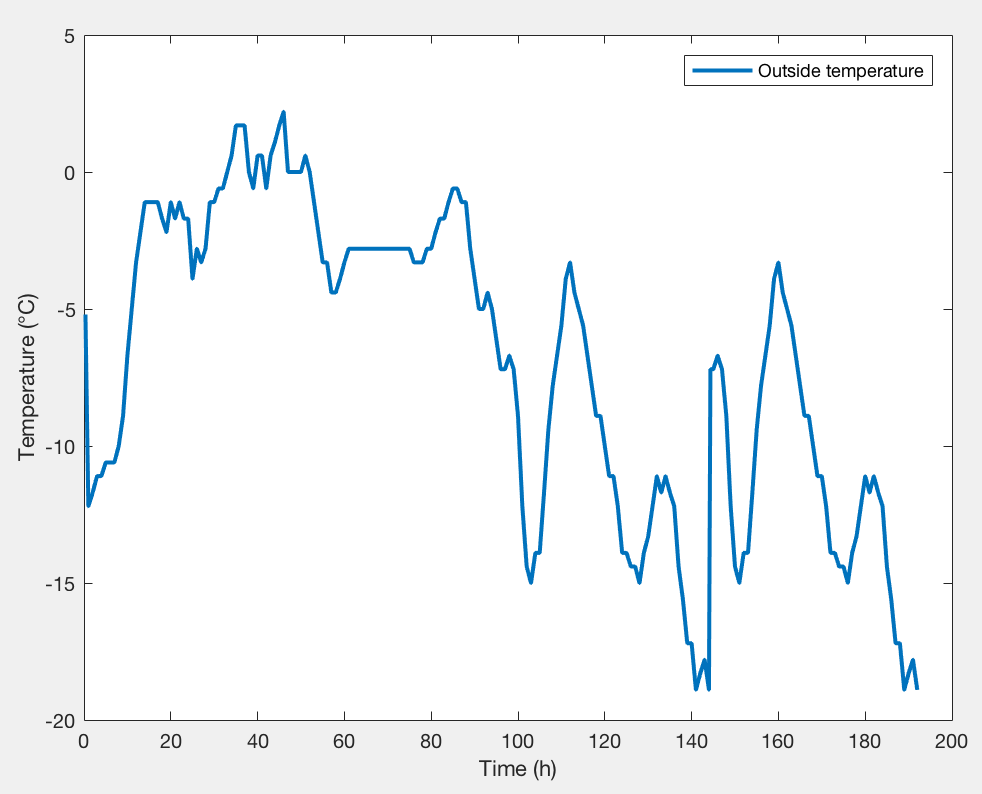
\includegraphics[width=\linewidth]{temp_pred}
				\caption{External temperature predictions}
				\label{fig::temp_pred}
			\end{minipage}
			\begin{minipage}{0.45\linewidth}
				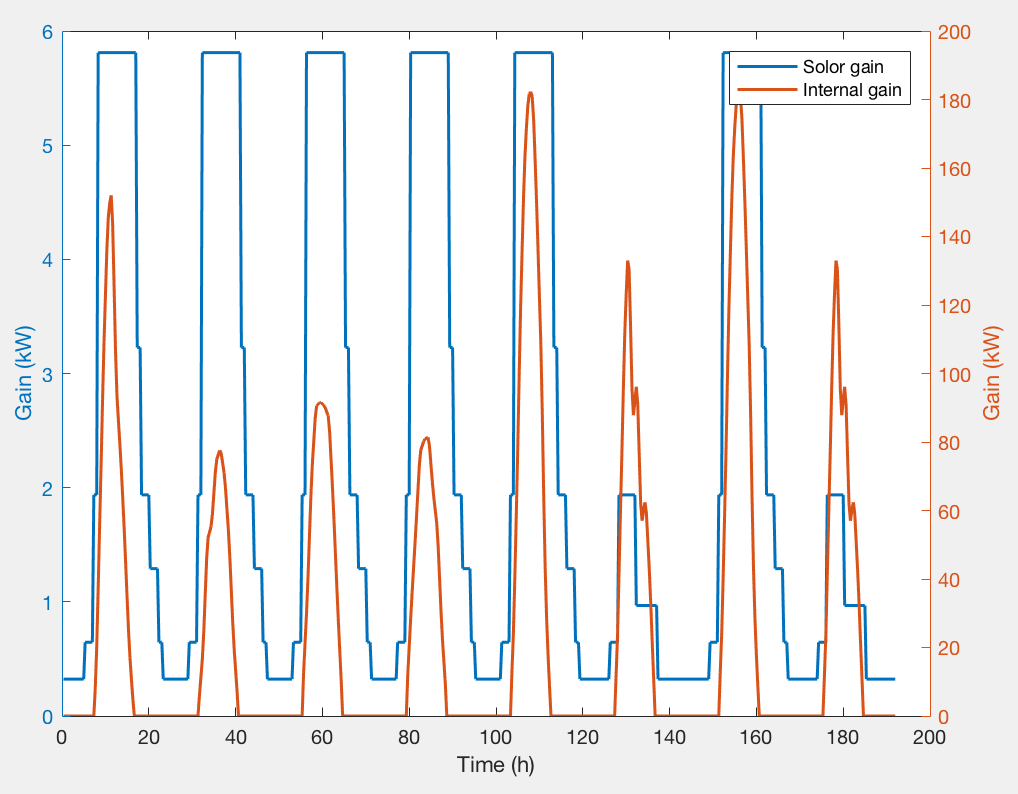
\includegraphics[width=\linewidth]{gains_pred}
				\caption{Solar and internal gain predictions}
				\label{fig::gain_pred}
			\end{minipage}
		\end{figure}
		
		\paragraph{} The following sections implements different versions of model predictive controllers, considering different objectives : target tracking, cost minimization, storage cost, .. 
	}
	
	\section{First MPC Controller}
	{
		\paragraph{} In this section, we are using YALMIP in order to design a MPC controller. This controller must regulate the output of the system around the reference output : 
		\begin{equation}
			y_r = \begin{pmatrix} 24 & 24 & 24 \end{pmatrix}
		\end{equation}
		by optimizing the cost function : 
		\begin{equation}
			J = \sum_{n=1}^N (y_n-y_r)^T R (y-y_n)
		\end{equation}
		under the following constraints : 
		\begin{equation}
			\begin{aligned}
				& y_n \geq 22, \quad & &n\in\{1,\hdots,N\} \\
				& y_n \leq 26, \quad & &n\in\{1,\hdots,N\} \\
				& u_n \leq 15, \quad & &n\in\{1,\hdots,N\} \\												& u_n \geq 0, \quad & &n\in\{1,\hdots,N\} \\
			\end{aligned}
		\end{equation}
		In the following, $R$ is chosen to be $\mathds{1}_3$ (hence we are penalizing equally any fluctuations around the target value, independently of the room). Given a cost function, multiplying $R$ by a scalar value won't have any effect on the optimal solution. 
		\newline We decided \emph{not to implement} a terminal cost nor terminal set constraints. This was mainly motivated by the fact that even with small horizons $N$, the system is \emph{experimentally} stable and recursively feasible. Hence, given the fact that the control invariant set could be computationally challenging to compute, and because its use would reduce the attraction zone in our state space, there was no real need to use terminal cost or terminal set. 
		
		\paragraph{} Figures (\ref{fig::naivempc_N5_output}) and (\ref{fig::naivempc_N5_inputs}) respectively show the dynamics of the outputs and inputs of the systems control this MPC controller, given a horizon $N=5$, along their respective constraints and reference. 
		
		\begin{figure}[ht!]
			\begin{minipage}{0.45\linewidth}
				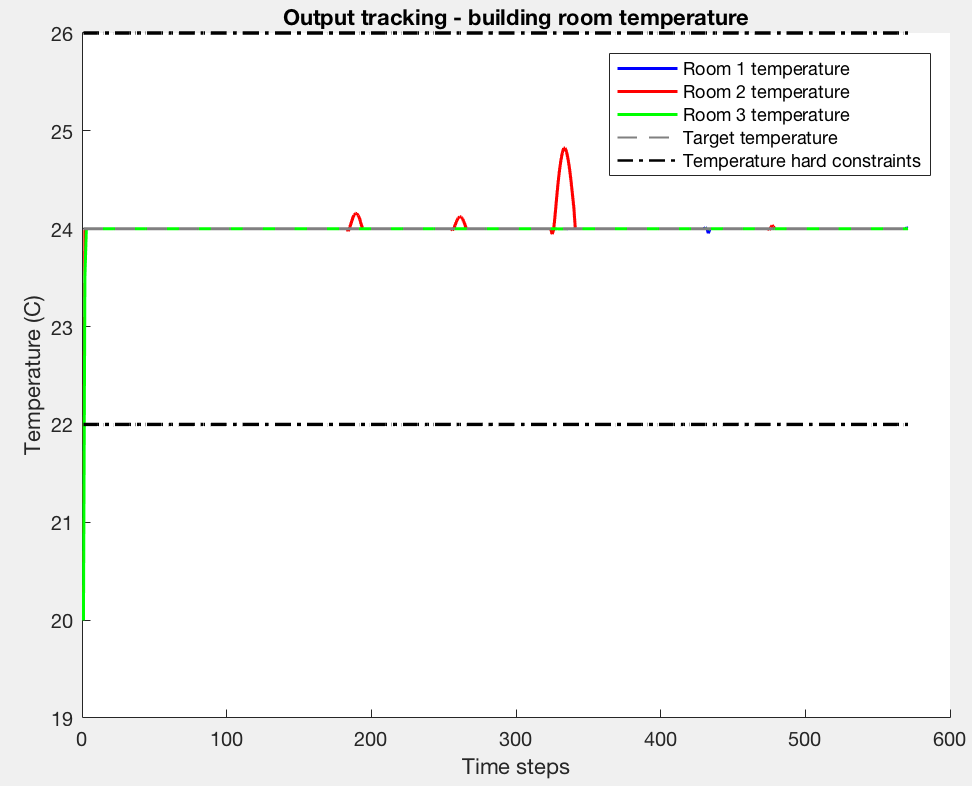
\includegraphics[width=\linewidth]{naivempc_N5_output}
				\caption{Output regulation, $N=5$}
				\label{fig::naivempc_N5_output}
			\end{minipage}
			\hfill
			\begin{minipage}{0.45\linewidth}
				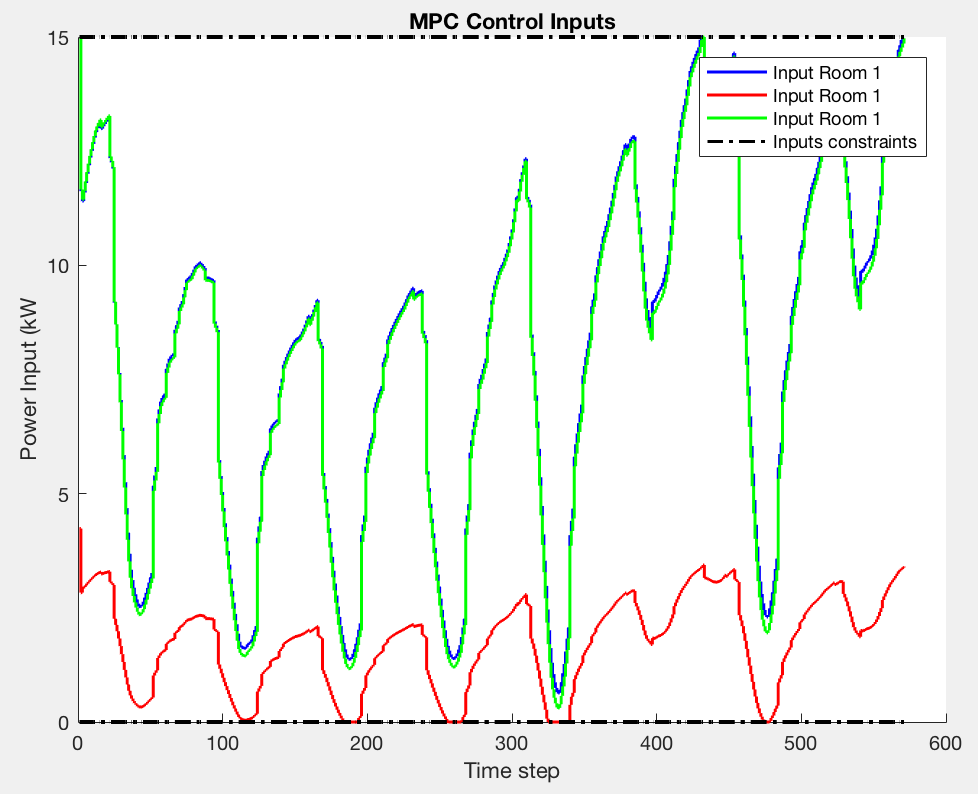
\includegraphics[width=\linewidth]{naivempc_N5_inputs}
				\caption{Inputs, $N=5$}
				\label{fig::naivempc_N5_inputs}
			\end{minipage}
		\end{figure}
		We can already note that all constraints are indeed verified. Because the disturbance is perfectly forecast (the disturbance applied is exactly the predicted one), the output tracking is done almost perfectly. We can indeed note that the temperature of the second room sometimes shows an overshoot. Because it is probably south-orientated, it is warmed up by the sun, which causes the room's temperature to rise, even if the input is zero. We can wonder what happens if we increase the prediction horizon so that the controller would be able to consider this raise in temperature. Figure (\ref{fig::naivempc_N20_output}) shows the rooms temperature for a controller of receeding horizon $N=20$. 
		\begin{figure}[ht!]
			\begin{center}
				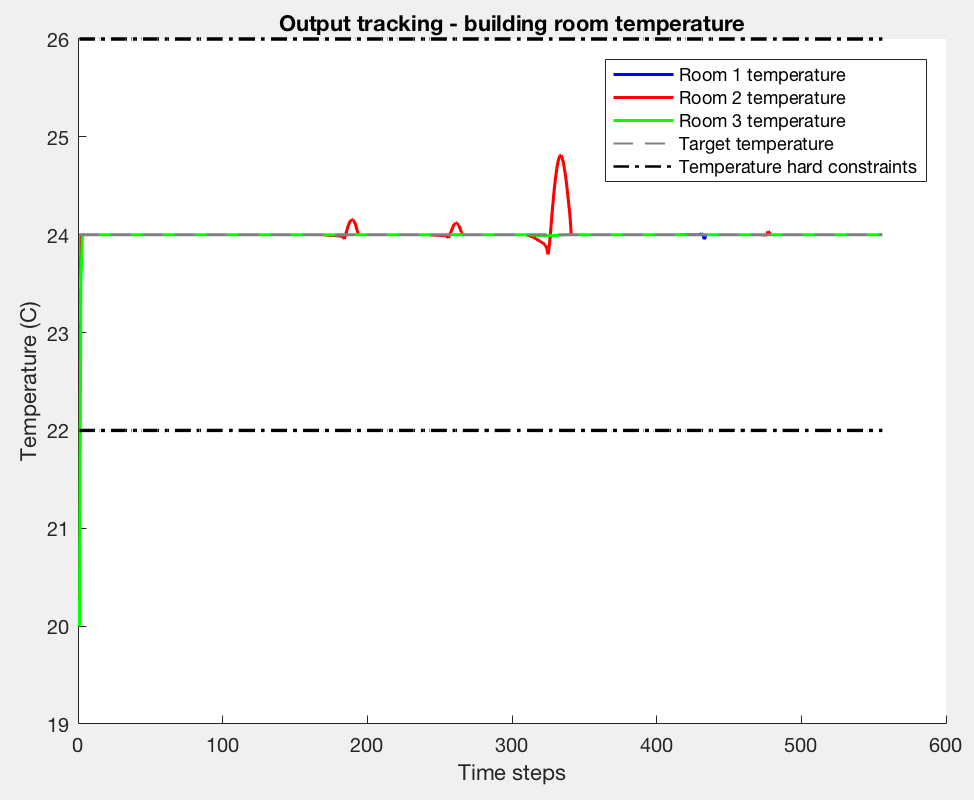
\includegraphics[width=0.5\linewidth]{naivempc_N20_output}
				\caption{Output regulation, $N=20$}
				\label{fig::naivempc_N20_output}
			\end{center}
		\end{figure}
		Because the controller is now able to consider the temperature raise due to the orientation of the room and the sun exposition, it allows a small undershoot by setting the corresponding input to 0 well before this event. Therefore, a smaller undershoot is achieved when increasing the horizon. 
	}
   
   	\section{Economic MPC}
	{
		\paragraph{} We now wish to formulate our objective function as an economic function : given the electricity's price, we would like to minimize our bill. 
		\paragraph{} This implies switching to a linear cost function : 
		\begin{equation}
			J = C^T\left(\sum_{n=1}^N u_n\right)
		\end{equation}
		where $C=\begin{pmatrix} c & c & c\end{pmatrix}^T$ is a cost matrix, with $c=0.2$ \$/kWh. However, this linear cost function might break some stability and recursive feasibility, which leads us to prefer a soft constraint formulation. 
	}
	
	\section{Soft Constraints}
	{
		\paragraph{} We decided to implement \emph{both} $L_2$ and $L_1$ penalization, in order to find a tradeoff between the amplitude of constraints violation and their duration. The actual optimization program we therefore solve writes : 
		\begin{mini}|s|[2]
  			{}{\sum_{n=1}^N\left[C^Tu_i +  \lVert \eps_n\rVert_2 +\lVert \eps_n\rVert_1 \right]}
  				 {\label{eq::svr}}{}
				 \addConstraint{y_n \geq 22}{\quad & &n\in\{1,\hdots,N\}}
				 \addConstraint{y_n \leq 26}{\quad & &n\in\{1,\hdots,N\}}
				 \addConstraint{u_n \leq 15}{\quad & &n\in\{1,\hdots,N\}}
				 \addConstraint{u_n \geq 0}{\quad & &n\in\{1,\hdots,N\}}
		\end{mini}
	}
\end{document}